Go言語の標準パッケージにはWebSocketに対するサポートはありません。しかしオフィシャルでメンテナンスされているgo.netサブパッケージにはこれに対するサポートがあります。以下のようなコマンドによってこのパッケージを取得することができます:


\begin{lstlisting}[numbers=none]
go get code.google.com/p/go.net/websocket
\end{lstlisting}

WebSocketはクライアントとサーバに分けられます。ここでは簡単な例を実現します:ユーザが情報を入力し、クライアントはWebSocketを通じて情報をサーバに送信します。サーバが情報を受け取った後主動的に情報をクライアントにPushします。クライアントは受け取った情報を出力します。クライアントのコードは以下のとおり:

\begin{lstlisting}[numbers=none]
<html>
<head></head>
<body>
    <script type="text/javascript">
        var sock = null;
        var wsuri = "ws://127.0.0.1:1234";

        window.onload = function() {

            console.log("onload");

            sock = new WebSocket(wsuri);

            sock.onopen = function() {
                console.log("connected to " + wsuri);
            }

            sock.onclose = function(e) {
                console.log("connection closed (" + e.code + ")");
            }

            sock.onmessage = function(e) {
                console.log("message received: " + e.data);
            }
        };

        function send() {
            var msg = document.getElementById('message').value;
            sock.send(msg);
        };
    </script>
    <h1>WebSocket Echo Test</h1>
    <form>
        <p>
            Message: <input id="message" type="text" value="Hello, world!">
        </p>
    </form>
    <button onclick="send();">Send Message</button>
</body>
</html>
\end{lstlisting}

クライアントのJSを見ると、WebSocket関数を使って簡単にサーバと接続するsockを作成することができると分かります。ハンドシェイクが成功した後、WebScoketオブジェクトのonopenイベントが呼ばれ、クライアントの接続の確立が成功したことを伝えます。クライアントでは4つのイベントを結びつけています。

\begin{enumerate}
  \item onopen 接続を確立すると呼ばれます
  \item onmessage 情報を受取ると呼ばれます
  \item onerror エラーが発生した時に呼ばれます
  \item onclose 接続を閉じた際に呼ばれます
\end{enumerate}

我々のサーバの実装は以下の通り:

\begin{lstlisting}[numbers=none]
package main

import (
    "golang.org/x/net/websocket"
    "fmt"
    "log"
    "net/http"
)

func Echo(ws *websocket.Conn) {
    var err error

    for {
        var reply string

        if err = websocket.Message.Receive(ws, &reply); err != nil {
            fmt.Println("Can't receive")
            break
        }

        fmt.Println("Received back from client: " + reply)

        msg := "Received:  " + reply
        fmt.Println("Sending to client: " + msg)

        if err = websocket.Message.Send(ws, msg); err != nil {
            fmt.Println("Can't send")
            break
        }
    }
}

func main() {
    http.Handle("/", websocket.Handler(Echo))

    if err := http.ListenAndServe(":1234", nil); err != nil {
        log.Fatal("ListenAndServe:", err)
    }
}
\end{lstlisting}

クライアントがユーザの入力した情報をSendした後、サーバはReceiveを通して対応する情報を受け取ります。その後Sendを通して応答情報を送信します。

\begin{figure}[H]
  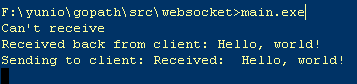
\includegraphics[width=7cm]{8.2.websocket3.png}
   \label{図8.4}
   \caption{WebSocketサーバが受け取った情報}
\end{figure}

上の例でクライアントとサーバでWebSocketを実装するのが非常に簡単だとわかりました。Goのソースコードのnetブランチではすでにこのプロトコルが実装されており、直接持ってきて使用することができます。現在HTML5の発展にしたがって将来WebSocketがWeb開発にとって重要になると考えています。我々はこの方面の知識を蓄える必要があります。


